\documentclass[10pt]{article}
\usepackage{charsheet}
\usepackage{multicol}
\usepackage{enumitem}
\usetikzlibrary{fit}
%\usepackage{amsmath}
\colorlet{grayed out}{white!70!black}

\newcommand\scrm[1]{\textrm{\textsc{#1}}}

\newcommand\bigstrut{\vrule width 0pt height 16pt depth 0pt }

\usepackage{pgfkeys}

\newlength\colwidth
\newlength\colgap
\colgap=10pt
\setlength\colwidth{(\textwidth-2\colgap)/3}
\dndrightwidth=\colwidth % XXX ugly

\newlength\hpwidth
\setlength\hpwidth{\colwidth-12pt}

\tikzset{%
  columnbox/.style={
    decorated stub rectangle,
    minimum width=\colwidth,
    draw, line width=1.2pt,
    label footer height=8pt,
  },
  initiative/.style={
    decorated clipped rectangle,
    minimum width=\hpwidth/3-10pt,
    draw, line width=1.2pt,
    fill=white,
    minimum height=18mm,
    label footer height=8pt,
  },
  dndhits/.style={
    dndmaxhp,
    minimum width=\hpwidth/2-5pt,
    minimum height=18mm,
    font=\footnotesize,
  }
}

\begingroup
  \tikzset{dndbox}%
  \pgfkeysgetvalue{/tikz/stub radius}{\srtmp}%
  \xdef\dndStubRadius{\srtmp}
\endgroup



\newsectionenv[width=\colwidth]{magic}{MAGIC}
  {\begin{minipage}[t]{\hsize}
   \featurespostspace=0pt
   \useDNDfont{MAGIC}
  }
  {\end{minipage}}
\newsectionenv[width=\colwidth]{attacks}{ATTACKS}{}{}
\newsectionenv[width=\colwidth]{features}{FEATURES}{}{}
\newsectionenv[width=\colwidth,decorated clipped rectangle]{equipment}{EQUIPMENT}
   {%
     \medskip
     \noindent
     \hspace*{21mm}%
     \begin{minipage}{\hsize-21mm}
     \ifnum\rawgetDND{EQUIPMENT COLS}=1
     \else
        \begin{multicols}{\rawgetDND{EQUIPMENT COLS}}
     \fi
     \small
      \begin{eqlist}%
     \ifDNDnonempty{EQUIPMENT}{}{%
       \item \noindent\vrule width 0pt height 0pt depth 8\baselineskip (Placeholder: Equipment will go here.)
     }%
   }
   {\end{eqlist}%
    \ifnum\rawgetDND{EQUIPMENT COLS}=1
    \else
       \end{multicols}
    \fi
    \end{minipage}%
   }


\newsectionenv[width=38mm]{proficiencies}{PROFICIENCIES}
   {\par\medskip
    \begin{minipage}[t]{34mm}
     \begin{proflist}}
   {\end{proflist}
    \end{minipage}}

  

\begin{document}


\newcommand\nextstatloc{inside north west corner=of stats background}


\input{stats}

\setDND{EQUIPMENT COLS}{1}

\noindent
\begin{charsheet}

  \node [dndfull,height=20mm,fill=playername,below=of top] (splash) 
     {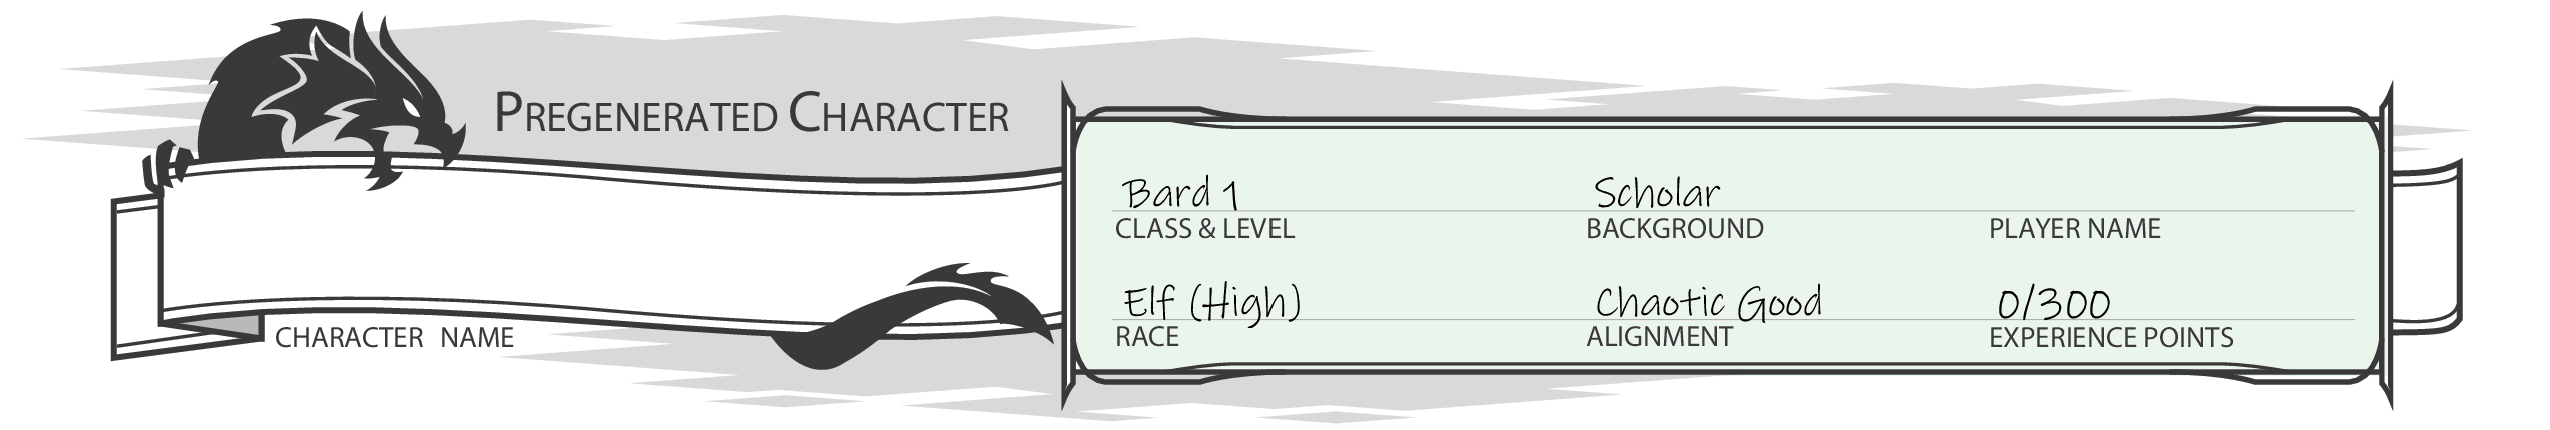
\includegraphics[width=\textwidth]{splash.png}};

  \colorlet{splashgray}{white!85.765!black}



  \begingroup\sffamily

  \newcommand\namestrut{\vrule width 0pt depth 1pt\relax}

  \path ($(splash.south west)+(88mm,18.75mm)$) coordinate  (class field sw);
  \path ($(splash.south west)+(88mm,9.7mm)$) coordinate  (race field sw);
  \path ($(splash.south west)+(48mm,16mm)$) coordinate  (charname center);
  \path ($(splash.south west)+(40mm,24mm)$) coordinate  (pregen left);
 

  \ifDNDfalse{PREGENERATED}%
    {\node [fill=splashgray,width=42mm,height=5mm,anchor=south west,at=(pregen left)] {};}
    {}


  \node [fill=splashfield,width=97mm,height=6mm,anchor=south west,at=(class field sw)] {};
  \node [fill=splashfield,width=97mm,height=6mm,anchor=south west,at=(race field sw)] {};

  \path (class field sw) +(0mm,0.6mm) coordinate (class sw);
  \path (race field sw) +(0mm,0.6mm) coordinate (race sw);

  \writesplash[at=(class sw)]{34mm}{CLASS + LEVEL}
  \writesplash[right of base=1mm of CLASS + LEVEL]{28mm}{BACKGROUND}
  \writesplash[right of base=1mm of BACKGROUND]{34mm}{PLAYER NAME}

  \writesplash[at=(race sw)]{34mm}{RACE}
  \writesplash[right of base=1mm of RACE]{34mm}{ALIGNMENT}
  \writesplash[right of base=1mm of ALIGNMENT]{34mm}{EXPERIENCE POINTS}

  \ifDNDdefined{CHARACTER NAME}
{\node[at=(charname center),font={\rmfamily\LARGE\itshape},anchor=center]
      {\getDND{CHARACTER NAME}\ifDNDnonempty{AGE}{ \Large (\getDND{AGE})}{}}
      ;
    }
    {}

\Large

      \node (hpbackground) 
        [outer sep=0pt,stub rectangle,fill=hpetc,below=5mm of splash.south,width=\colwidth, minimum height=86mm] 
       { };

      \node (initiative)
            [initiative,below=of hpbackground.north,dndlabel=\noexpand\footnotesize INITIATIVE] 
         {\getDND*{INITIATIVE}}
         ;

       \node (ac) [initiative,shield,innershield,draw,ultra thick,left=of initiative,width=15mm,
                   dndlabel={\noexpand\tinystacklabel{ARMOR}{CLASS}},
                   font=\Large,
                   label footer height=12pt,
            ]
      {\getDND*{ARMOR CLASS}}
      ;

      \node (speed)
            [initiative,right=of initiative,dndlabel=SPEED] 
         {\getDND*{SPEED}}
         ;

      \node [dndmaxhp,below=of initiative,dndlabel=CURRENT HIT
             POINTS,minimum height=20mm,width=\hpwidth] 
         (maxhp)
         {}
         ;
      \node [below=of maxhp.north,font=\scriptsize] {%
         \hbox to \hpwidth{%
             ~~~Maximum Hit Points~~\rlap{\raisebox{4pt}{\smash{\normalsize~~~\getDND*{MAX HP}}}}%
               \hrulefill~~~}}
       ;

      \node[dndmaxhp,below=of maxhp,minimum height=20mm,width=\hpwidth,dndlabel=TEMPORARY HIT POINTS]
        (temphp)
        {}
        ;



      \node (hitdice)
             [dndhits,below left corner=of temphp,
             dndlabel=HIT DICE,label footer height=-2pt,
             font=\Large] 
         {\getDND*{HIT DICE}}
         ;

     \ifDNDdefined{LEVEL}{
         \node [at=(hitdice.north),anchor=north] 
              {\expandafter\stackslots\expandafter{\rawgetDND{LEVEL}+1}};
     }{}

      \node (death saves)
            [dndhits,fill=white,below right corner=of temphp,
             dnd/label={DEATH SAVES},font=\small] 
         { \tiny\begin{tabular}{@{}r@{\hskip1pt}l@{}}
            \raisebox{1pt}{SUCCESSES}&\slotsliteral3\\[2pt]
            \raisebox{1pt}{FAILURES}&\slotsliteral3\\
            \end{tabular}
          }
         ;


%\node [draw,above=of initiative] % {\slotsliteral7};
%              {\expandafter\stackslots\expandafter{\rawgetDND{LEVEL}+1}};





  \endgroup


\makeatletter
\renewcommand\attackkeys[1]{%
  \gdef\@attackname{}%
  \gdef\@attackattack{}%
  \gdef\@attackdamage{}%
  \gdef\@attacktype{}%
  \gdef\@attackrange{}%
  \gdef\@attackammo{}%
  \pgfkeys{/attacks/.cd, #1}%
  \small \@attackname&\@attackattack&\@attackdamage\ \small\@attacktype\\
}
\makeatother


\newdimen\attacksInnerSep
\attacksInnerSep=4pt



\node[columnbox,anchor=north east,dndlabel=Description \&\ Personality,
      inner sep=10pt,
    ] (motivation) at (splash.east |- hpbackground.north)
   {\begin{minipage}{\colwidth-22pt}
    \newcommand\hangpar{\hangindent=1em \hangafter=1 \par}
    \smallskip
    Motivation:\\
    \getDND*{MOTIVATION}
    \hangpar
    \bigskip
    \ifDNDnonempty{SUGGESTED MOTIVATIONS}{%
       Suggested Motivations:\\ \getDND{SUGGESTED MOTIVATIONS} \hangpar
       \bigskip
    }{}
    \ifDNDnonempty{SUGGESTED NAMES}{%
       Suggested Names:\\ \getDND{SUGGESTED NAMES} \hangpar
       \bigskip
    }{}
    \hbox{}
   \end{minipage}
   }
;


\newenvironment{itemize spells}
  {\clubpenalty=10000
   \widowpenalty=10000
   \begin{itemize}[topsep=0pt,itemsep=0pt,leftmargin=6pt,parsep=0pt,labelsep=2pt]
  }%
  {\end{itemize}}

\path (motivation.south west) ++(0mm, -3mm) coordinate (features upper fit);


\ifDNDdefined{FEATURES}{
  \begin{features}[fit=(bottom right)(features upper fit),dndlabel=FEATURES \&\ TRAITS]{}
  \raggedright
  \def\described#1#2{\strut\emph{#1:} #2\par\smallskip}%
  \getDND{FEATURES}

  \ifDNDnonempty{MAGIC}{%
    \smallskip
    \footnotesize
    \newcommand\spellslevellabel[2]{%
      \ifnum#1=0
         Cantrips: You can cast these spells as often as you like using 1~action.
      \else
         \end{itemize spells}
         Level~#1 spells: Cast these spells in any combination%
         \ifnum#2>0\relax
            \ #2~times per long rest.
         \else
            .
         \fi
        Casting is 1~action unless noted.
      \fi
      \begin{itemize spells}
    }
    \def\described#1#2{\item #1: #2}%
    \getDND{MAGIC}
    \end{itemize spells}
  }{}%
  \end{features}
}{}

\node (stats background) 
      [fill=stats,width=24mm,height=163mm,anchor=north west]
      at (splash.west |- hpbackground.north)
 { };

\dndstat{STRENGTH}{STR}
\dndstat{DEXTERITY}{DEX}
\dndstat{CONSTITUTION}{CON}
\dndstat{INTELLIGENCE}{INT}
\dndstat{WISDOM}{WIS}
\dndstat{CHARISMA}{CHA}



% slots OK here

\node (inspiration)
      [fill=white,draw,line width=1.2pt,decorated stub rectangle,width=38.001mm,height=8mm,
       right of upper corner=5mm of stats background]
   {\hbox to 0pt{\hss\hspace*{6mm}\small\textsf{INSPIRATION}\hss}}
   ;
\node [anchor=west,proficiencies,fill=white,decorated stub rectangle,
       width=10mm,height=10mm,line width=1.5pt,draw]
       at ($(inspiration.west)+(-2mm,0mm)$)
      {};

\node[columnbox,width=38.002mm,dndlabel=SAVING THROWS,
      fill=white,below=4mm of inspiration,
      height=35mm,
    ]
    (saving throws)
    {\begin{tabular}{l@{ \vrule width 20pt height 0pt depth 0.2pt\ }l}
      \(\circ\)&Strength\\
      \(\circ\)&Dexterity\\
      \(\circ\)&Constitution\\
      \(\circ\)&Intelligence\\
      \(\circ\)&Wisdom\\
      \(\circ\)&Charisma\\
    \end{tabular}}
  ;
\node (proficiency bonus)
      [proficiencies,decorated stub rectangle,width=38.001mm,height=8mm,
       below=6mm of saving throws]
   {\hbox to 0pt{\hss\hspace*{6mm}\tiny\textsf{PROFICIENCY BONUS}\hss}}
   ;
\node [anchor=west,proficiencies,circle,
       width=10mm,height=10mm,line width=1.5pt,draw]
       at ($(proficiency bonus.west)+(-2mm,0mm)$)
      {\large\textsf{+\arabic{proficiency bonus}}};

\path (inspiration.south |- stats background.south) coordinate (prof bot fit);
\path (proficiency bonus.south) ++ (0,-5mm) coordinate (prof top fit);

% Proficiencies section (middle top)
\begin{proficiencies}[width=38.002mm,height=2in,inner sep=0pt,
                      fit=(prof bot fit)(prof top fit -| saving throws.west)(prof top fit -| saving throws.east)]
  \small
\ifDNDdefined{PROFICIENCIES}{%
{\tracingmacros=1
  \long\def\split#1\profskip#2\nil{%
    \def\profbefore{#1}% before part
    \def\profafter{#2}%  after part (empty if no \profskip in input)
  }
  \expandafter\expandafter\expandafter\expandafter\expandafter\expandafter\expandafter\split\rawgetDND{PROFICIENCIES}\profskip\nil
  \profbefore
  \expandafter\gdef\expandafter\otherproficiencies\expandafter{\profafter}%
%  \expandafter\def\expandafter\theprofs\expandafter{\rawgetDND{PROFICIENCIES}}%
%  \expandafter\profskipCar\expandafter{\theprofs}%
}%
}{%
  (None specified)
}
\end{proficiencies}

%\node (motivation) [below=of proficiencies] 
%  {\parbox{36mm}{\Large\centering\textit{\getDND*{MOTIVATION}}}}
%  ;

\path (hpbackground.south |- features.south) coordinate (bottom center);

\ifDNDdefined{EQUIPMENT}{%
%  \typeout{equipment, not magic}%
  {%
%  \begin{equipment}[fit=(equipment upper left fit)(equipment upper
%  right fit)(current bounding box.south)]
  \begin{equipment}[height=124pt,width=\colwidth,anchor=south,at=(bottom center)]
     \useDNDfont{EQUIPMENT}%
     \getDND{EQUIPMENT}
  \end{equipment}
  }
}
{\node (equipment) [left of lower corner=of features] {};
}

\path (equipment.south west) +(5mm,40mm) coordinate (coin top left);


\coin{cp}{Cu}{\color{grayed out}\getDND*{CP}}
\coin{sp}{Ag}{\color{grayed out}\getDND*{SP}}
\coin{gp}{Au}{\color{grayed out}\getDND*{GP}}
\coin{pp}{Pt}{\color{grayed out}\getDND*{PP}}
  
\newenvironment{attackstab*}
  {\renewcommand\arraystretch{1.3}%
   \def\notesheader{\multicolumn6{@{}l}{\vrule width 0pt height 18pt\small\textsf{\textit{NOTES}}}\\}%
   \tabcolsep=0.5\tabcolsep
   \normalsize
   \let\dndkeys=\attackkeys
   \noindent
   \hspace*{\attacksInnerSep}%   
   \begin{tabular*}{\hsize-2\attacksInnerSep}{@{}lll@{}}
   \textsf{\footnotesize NAME}&
   \textsf{\scriptsize \llap{ATK BO}NUS}&
   \textsf{\scriptsize DAMAGE/TYPE}\\
   \midrule
  }
  {\end{tabular*}\hspace*{\attacksInnerSep}\par}

\path (hpbackground.south west) ++(\dndStubRadius, -4mm) coordinate (attacks upper left fit);
\path (equipment.north east) ++(-\dndStubRadius, 4mm) coordinate (attacks lower right fit);

\begin{attacks}[fit=(attacks upper left fit)(attacks lower right fit)]{}
    \centering
    \begin{attackstab*}
    \getDND{ATTACKS}
    \end{attackstab*}

    \medskip

    \begin{minipage}{\hsize-2\attacksInnerSep}
    \DNDranges
    \end{minipage}
    \vfill
\end{attacks}

\node (motivations) [above=4.45mm of BACKGROUND.north] 
  {\Large\textit{\getDND*{MOTIVATION}}}
  ;


\node [anchor=south west,columnbox,minimum height=45mm,
       dndlabel={Weapon, Armor, \&\ Language Proficiencies},
      ]
   (other proficiencies)
   at (bottom left |- features.south)
  {\begin{minipage}[t]{\colwidth-10pt}
    \begin{multicols}{2}
    \begin{proflist}
    \itemsep=1pt
    \otherproficiencies
    \end{proflist}
    \end{multicols}
  \end{minipage}
  }
  ;

\node (passive perception)
      [decorated stub rectangle,width=\colwidth-8mm,height=8mm,
       line width=1.2pt,draw,
       above right corner=5mm of other proficiencies]
   {\hbox to 0pt{\hss\footnotesize\textsf{PASSIVE WISDOM (PERCEPTION)}\hss}}
   ;

\node [anchor=east,circle,fill=white,
       width=10mm,height=10mm,line width=1.5pt,draw]
       at ($(passive perception.west)+(+2mm,0mm)$)
      {\ifDNDnonempty{PASSIVE PERCEPTION}
         {\large\textsf{\signed{\rawgetDND{PASSIVE PERCEPTION}}}}
         {?}
      }
      ;


%\node [draw,below=of initiative] % {\slotsliteral7};
%              {\expandafter\stackslots\expandafter{\rawgetDND{LEVEL}+5}};


\firsttwoDNDnonempty{\upperdndlabel}{\upperdndcontents}{\lowerdndlabel}{\lowerdndcontents}{SORCERY POINTS,SENSES,SPELL DC,PASSIVE PERCEPTION}

%\typeout{upper is \upperdndlabel; lower is \lowerdndlabel}

%{\ifDNDnonempty{SENSES}{\typeout{SENSES IS NOT EMPTY; it is !\rawgetDND{SENSES}!}}{}}

%\node [draw,below=of maxhp] % {\slotsliteral7};
%              {\expandafter\stackslots\expandafter{\rawgetDND{LEVEL}+1}};

% slots not OK here


%\ifDNDdefined{SPELL DC}
%  {
%      \node (spell dc)
%         [dndmaxhp,left=10mm of maxhp,width=24mm] 
%         {\Large\textsf{13}}
%         ;
%
%      \dndlabel{spell dc}{SPELL DC}
%  }
%  {
%      \node (passive perception)
%         [dndmaxhp,left=10mm of maxhp,width=24mm] 
%         {\Large\textsf{\getDND*{PASSIVE PERCEPTION}}}
%         ;
%
%      \dndlabel{passive perception}{\pplabel}
%  }
%
%\node (senses)
%   [dndmaxhp,left=10mm of curhp,width=24mm] 
%%   {\itshape\begin{tabular}{c}{Darkvision}\\{60~ft}\\[3pt]\end{tabular}}
%   {\parbox{20mm}{\centering\itshape\getDND*{SENSES}}}
%   ;
%\dndlabel{senses}{\scriptsize SENSES}
%
%

\def\sp{SORCERY POINTS}
\ifx\upperdndlabel\sp
  \edef\upperdndcontents{\noexpand\stackslots{\rawgetDND{SORCERY POINTS}}}%
\fi

\def\se{SENSES}
\ifx\upperdndlabel\se
  \def\upperdndcontents{\parbox{20mm}{\centering\rmfamily\small\textit{\getDND{SENSES}}}}%
\fi

%\show\pp
%%\show\upperdndlabel
%
%  \node (upper val)
%         [dndmaxhp,left=10mm of maxhp,width=24mm] 
%         {\Large\textsf{\upperdndcontents}}
%         ;
%
%      \ifDNDfont{\upperdndlabel}
%         {\dndlabel[\upperdndlabel]{upper val}{\upperdndlabel}}
%         {\dndlabel{upper val}{\upperdndlabel}}
%
%\ifx\lowerdndlabel\empty\else
%
%   \node (lower val)
%      [dndmaxhp,left=10mm of curhp,width=24mm] 
%      {\Large\textsf{\lowerdndcontents}}
%      ;
%      \ifDNDfont{\lowerdndlabel}
%         {\dndlabel[\lowerdndlabel]{lower val}{\lowerdndlabel}}
%         {\dndlabel{lower val}{\lowerdndlabel}}
%
%\fi


%\node [draw,above=of features] {\parbox{4in}{7 slots: minimum \minrows{7} rows\par \stackslots7\par\hbox{\slotsliteral3}}};


\end{charsheet}

% Equipment Weight Summary Page
\clearpage

\begin{charsheet}

\sffamily


% Define colors for capacity boxes
\colorlet{carrying}{white}
\colorlet{encumbered}{proficiencies}  % Use existing yellow from charsheet.sty
\colorlet{heavilyencumbered}{magic}   % Use existing red from charsheet.sty
\colorlet{unencumbered}{equipment}

% Define height per tenth of stone for equipment slots
\newdimen\tenthstoneheight
\tenthstoneheight=8pt

% Calculate carrying capacity thresholds (in tenths of stones)
\newcounter{carryingCapacity}
\newcounter{encumberedThreshold}
\newcounter{heavilyEncumberedThreshold}

\ifDNDnonempty{STR}{%
  % Carrying capacity = STR score in stones (convert to tenths)
  \setcounter{carryingCapacity}{\numexpr\rawgetDND{STR} * 10\relax}
  
  % Encumbered = 1/3 of carrying capacity, rounded down
  \setcounter{encumberedThreshold}{\numexpr\rawgetDND{STR} * 10 / 3\relax}
  
  % Heavily encumbered = 2/3 of carrying capacity, rounded down  
  \setcounter{heavilyEncumberedThreshold}{\numexpr\rawgetDND{STR} * 20 / 3\relax}
}{%
  % No STR defined - leave counters at zero
}

\node (banner) [below=of top]
      {\LARGE{\textsf{\textbf{Equipment and Encumbrance by Stones%
        \ifDNDnonempty{CHARACTER NAME}{ (\getDND{CHARACTER NAME})}{}}}}};

% Calculate total weight (in tenths of stones)
\newcounter{significantWeight}
\withitemweight{\setcounter{significantWeight}}{HEAVY WEAPONS}
\withitemweight{\addtocounter{significantWeight}}{NORMAL WEAPONS}
\withitemweight{\addtocounter{significantWeight}}{SHIELDS}
\withitemweight{\addtocounter{significantWeight}}{HEAVY ARMOR}
\withitemweight{\addtocounter{significantWeight}}{MEDIUM ARMOR}
\withitemweight{\addtocounter{significantWeight}}{LIGHT ARMOR}
\withitemweight{\addtocounter{significantWeight}}{HEAVY ITEMS}

\newcounter{remainingCapacity}
\ifDNDnonempty{STR}{%
  % Remaining = carrying capacity - significant weight (in tenths of stones)
  \setcounter{remainingCapacity}{\numexpr\rawgetDND{STR} * 10 - \value{significantWeight}\relax}
  % Convert to stones and multiply by 5 for line count
  \setcounter{remainingCapacity}{\numexpr\value{remainingCapacity} * 5 / 10\relax}
}{%
  \setcounter{remainingCapacity}{0}
}

% Equipment slots box on the left with three-color backgrounds
% First calculate positions for color transitions in terms of \tenthstoneheight
\newcounter{greenLines}
\newcounter{yellowLines}  
\newcounter{redLines}

\ifDNDnonempty{STR}{%
  % Calculate how many lines each color region should have
  % Total lines = 5 * remaining capacity (in stones)
  % Use PGF arithmetic for truncation instead of \numexpr rounding
  % \pgfmathtruncatemacro truncates toward zero, giving us floor division for positive numbers

  %% use at most 43 slots
  \pgfmathtruncatemacro{\greenlines}{
    min(43, floor(((\value{encumberedThreshold}-\value{significantWeight})*5)/10))
  }
  % Clamp yellow to what's left
  \pgfmathtruncatemacro{\yellowlines}{
    max(0, min(43-\greenlines, floor(((\value{heavilyEncumberedThreshold}-\value{significantWeight})*5)/10)))
  }
  % Clamp red to what's left after green+yellow
  \pgfmathtruncatemacro{\redlines}{
    max(0, min(43-\greenlines-\yellowlines, ((\value{carryingCapacity}-\value{heavilyEncumberedThreshold})*5)/10))
  }
  \setcounter{greenLines}{\greenlines}
  \setcounter{yellowLines}{\yellowlines}
  \setcounter{redLines}{\redlines}
}{%
  \setcounter{greenLines}{0}%
  \setcounter{yellowLines}{0}%
  \setcounter{redLines}{0}%
}

% Calculate heights for each color region
\newdimen\greenheight
\newdimen\yellowheight
\newdimen\redheight

\greenheight=\numexpr2*\value{greenLines}\relax\tenthstoneheight
\yellowheight=\numexpr2*\value{yellowLines}\relax\tenthstoneheight  
\redheight=\numexpr2*\value{redLines}\relax\tenthstoneheight


\path (top left) 
 ++(0, -13mm)
  node (slotstitle)
    [slotblock,anchor=north west,fill=blue!10!white,minimum height=28pt] 
  {\Large\textbf{Slotted Items}}
  ;

% Three capacity boxes centered below top
\path (slotstitle.north east) ++(20pt,0)
 node (carrying) [dndencumbrance,fill=carrying,anchor=north west,dndlabel=CARRYING CAPACITY]
  {\Large\ifDNDnonempty{STR}{$\mathbf{\leq\renderstones{\arabic{carryingCapacity}}}$}{}};

\node (encumbered) [dndencumbrance,fill=encumbered,right=5mm of carrying,dndlabel=ENCUMBERED] 
  {\Large\ifDNDnonempty{STR}{$\mathbf{\geq\renderstones{\arabic{encumberedThreshold}}}$}{emptyb
  STR?}};

\node (heavily) [dndencumbrance,fill=heavilyencumbered,right=5mm of encumbered,dndlabel=HEAVILY ENCUMBERED]
  {\Large\ifDNDnonempty{STR}{$\mathbf{\geq \renderstones{\arabic{heavilyEncumberedThreshold}}}$}{}};


\node (e warning) [below=of encumbered] {\small(Speed drops by 10~ft)};
\node (h warning) [below=of heavily,inner sep=2pt] {%
  \hspace*{3mm}%
  \begin{minipage}{40mm}\raggedright
   \small
   (Speed drops by 20~ft;
   Disadvantage on ability checks, saving throws, and attack rolls that use \scrm{str}, \scrm{dex}, or \scrm{con}.)
   \end{minipage}}
  ;


\path (slotstitle) coordinate (slotsbottom);

\ifdim\greenheight>0pt

  \node (slotgreen) [slotblock,fill=unencumbered,anchor=north west,
                     minimum height=\greenheight]
    at (slotstitle.south west) {} ;

  \path (slotgreen.south west) coordinate (slotsbottom);


  \ifdim\yellowheight>0pt

     \node (slotyellow) [slotblock,fill=encumbered,anchor=north west,
                        minimum height=\yellowheight]
       at (slotgreen.south west) {} ;

     \path (slotyellow.south west) coordinate (slotsbottom);


     \ifdim\redheight>0pt

        \node (slotred) [slotblock,fill=heavilyencumbered,anchor=north west,
                           minimum height=\redheight]
          at (slotyellow.south west) {} ;

        \path (slotred.south west) coordinate (slotsbottom);



     \fi
  \fi
\fi

\foreach \deltay in {1,2,...,\numexpr\value{greenLines}+\value{yellowLines}+\value{redLines}\relax} {
  \draw (slotstitle.south west)
    ++(8pt,-\deltay*2*\tenthstoneheight)
    -- ++(\slotblockwidth-16pt,0)
   ;
}

\path (slotstitle.south west) ++(5pt,2pt) coordinate (lastslot);

\begingroup
  \newcommand\DNDitem[2]{%
     \path (lastslot)
       ++(0,-2\tenthstoneheight)
       node [anchor=base west] (thisslot) {\color{grayed out}#1};
     \path (thisslot.base west) coordinate (lastslot);
  }
  \doDNDitems{LIGHT WEAPONS}
  \doDNDitems{SLOTTED ITEMS}
\endgroup

\path (slotsbottom) ++(1pt,2pt) coordinate (decor ll)
      (slotstitle.north east) ++(-1pt,-2pt) coordinate (decor ur)
  ;

\node [draw,decorated stub rectangle,thick,
    stub radius=2.3mm,
    line width=1.2pt,
        fit=(decor ll) (decor ur),
      ]
  (slots decoration)
  {};


%
%  \foreach \thing in {{fish},{fowl},{fury}} {
%     \node [anchor=north] at (lastslot.south) (thisslot) {\thing};
%     \path (thisslot.south) coordinate (lastslot);
%  }
%


%%%%    \node [dndbox,slotblock,below=5mm of heavy equipment,fill=equipment,inner sep=15pt] 
%%%%       (worn items)
%%%%    {
%%%%      \def\arraystretch{1.32}%
%%%%    %  \newcommand{\DNDitem}[2]{#1&$\mathbf{\renderstones{#2}}$&\stonesplural{#2}\crcr}%
%%%%      \newcommand{\DNDitem}[2]{#1\crcr}%
%%%%      \begin{tabular}{l}
%%%%      \multicolumn1{c}{\bigstrut \Large \textbf{Worn Items}}\\[5pt]
%%%%      % Local definition of \DNDitem for display
%%%%      % Display all significant equipment items
%%%%      \doDNDitems{WORN ITEMS}%
%%%%    %  Z\crcr
%%%%    %  \midrule
%%%%    %  \doDNDitems{SLOTTED ITEMS}%
%%%%    %  Total&$\mathbf{\renderstones{\value{significantWeight}}}$&\stonesplural{\value{significantWeight}}\\
%%%%      \end{tabular}%
%%%%    };

%\path (heavily.east |- h warning.south) coordinate (h warning r);

\node [dndbox,slotblock,anchor=south east,at=(heavily.east |- slots decoration.south),
       fill=equipment,minimum height= 74\tenthstoneheight]
  (small items)
  { }
;

\node [below top=5mm of small items,minimum width=\slotblockwidth] (smalltitle) {\Large\textbf{Small Items}};

\foreach \deltay in {1,2,...,34} {
  \draw (smalltitle.south west)
    ++(12pt,-\deltay*2*\tenthstoneheight)
    -- ++(\slotblockwidth-24pt,0)
   ;
}

\begingroup
  \path (smalltitle.south west) ++(9pt, 2pt) coordinate (lastslot);
  \newcommand\DNDitem[2]{%
     \path (lastslot)
       ++(0,-2\tenthstoneheight)
       node [anchor=base west] (thisslot) {\color{black!30!white}#1};
     \path (thisslot.base west) coordinate (lastslot);
  }
  \doDNDitems{SMALL ITEMS}
\endgroup


% Equipment weight breakdown table
\node [dndbox,anchor=north west,at=(carrying.west |- small items.north),fill=equipment,inner sep=15pt] 
   (heavy equipment)
{
  \def\arraystretch{1.32}%
  \newcommand{\DNDitem}[2]{#1&$\mathbf{\renderstones{#2}}$&\stonesplural{#2}\\}%
  \begin{tabular}{lr@{~}l}
  \multicolumn3{c}{\bigstrut \Large \textbf{Heavy Equipment}}\\[5pt]
  \doDNDitems{HEAVY WEAPONS}%
  \doDNDitems{NORMAL WEAPONS}%
  \doDNDitems{SHIELDS}%
  \doDNDitems{HEAVY ARMOR}%
  \doDNDitems{MEDIUM ARMOR}%
  \doDNDitems{LIGHT ARMOR}%
  \doDNDitems{HEAVY ITEMS}%
  \midrule
  Total&$\mathbf{\renderstones{\value{significantWeight}}}$&\stonesplural{\value{significantWeight}}\\
  \end{tabular}%
};




\node [slotblock,anchor=south west,inner sep=0pt]
  at (slots decoration.south -| heavy equipment.west)
  {\Large\begin{tabular}{@{}l@{ = }l@{}}
   1 Slot &Bundle of up to 20\\
   \multicolumn1{@{}l@{}}{}&identical items, \emph{or}\\[3pt]
   \multicolumn1{@{}l@{}}{}&150~coins, \emph{or}\\[3pt]
   \multicolumn1{@{}l@{}}{}&1 stowed weapon\\[8pt]
   5 Slots&1 Stone\\
  \end{tabular}}
;
   


  
\end{charsheet}

\ifDNDfalse{VALIDATION ERRORS}{}
{
\section{Validation errors}
\begin{itemize}
\getDND{VALIDATION ERRORS}
\end{itemize}
}

\end{document}
